\documentclass[12pt]{article}
\usepackage[margin=1.2in]{geometry}
\usepackage[all]{nowidow}
\usepackage[hyperfigures=true, hidelinks, pdfhighlight=/N]{hyperref}
\usepackage[separate-uncertainty=true,group-digits=false]{siunitx}
\usepackage{graphicx,amsmath,physics,tabto,float,amssymb,pgfplots,verbatim,tcolorbox}
\usepackage{listings,xcolor,subfig,keyval2e,caption,import}
\numberwithin{equation}{section}
\numberwithin{figure}{section}
\numberwithin{table}{section}
\definecolor{stringcolor}{HTML}{C792EA}
\definecolor{codeblue}{HTML}{2162DB}
\definecolor{commentcolor}{HTML}{4A6E46}
\lstdefinestyle{appendix}{
    basicstyle=\ttfamily\footnotesize,commentstyle=\color{commentcolor},keywordstyle=\color{codeblue},
    stringstyle=\color{stringcolor},showstringspaces=false,numbers=left,upquote=true,captionpos=t,
    abovecaptionskip=12pt,belowcaptionskip=12pt,language=Python,breaklines=true,frame=single}
\lstdefinestyle{inline}{
    basicstyle=\ttfamily\footnotesize,commentstyle=\color{commentcolor},keywordstyle=\color{codeblue},
    stringstyle=\color{stringcolor},showstringspaces=false,numbers=left,upquote=true,frame=tb,
    captionpos=b,language=Python}
\renewcommand{\lstlistingname}{Appendix}
\pgfplotsset{compat=1.17}

\title{Hall Effect}
\author{KDSMIL001 \; PHY2004W PHyLAB 2}
\date{\textbf{17 November 2020}}

\begin{document}
    \begin{titlepage}
        \maketitle
        \center
        \tableofcontents
    \end{titlepage}
    
    \section{Introduction}\label{sec:Introduction}
    The Hall Effect is a well known effect that tells us a lot about the way that electric 
    charge conducts in materials. We will use it to determine some properties of the material 
    we're using, which is the p-type semiconductor germanium. 

    \section{Theory}\label{sec:Theory}
    If we have a block of material that conducts electricity and we put some current through it 
    there will be some kind of charge carrier moving through the material. Depending on the 
    material this could be either electrons, which are negatively charged, or positively charged 
    ''holes". If the material in question is placed within a magnetic field these moving charges 
    will feel a force in a direction perpendicular to their movement, dictated by 
    \begin{equation}
        \vec{F}=q\vec v\times\vec B
        \label{eqn:Lorentz Force}
    \end{equation}
    Because this force is perpendicular to the direction of movement of the charge carriers, we 
    will see some charge build-up on one side of the material, and a lack of charge on the other. 
    This means we can measure the voltage drop across the sides of the material. This voltage 
    is governed by the equation
    \begin{equation}
        V_\perp=R_H I_S B/c
        \label{eqn:V Perp}
    \end{equation}
    where $B$ is the strength of the magnetic field, $I_S$ is the applied current, and 
    $R_H\equiv \frac{1}{nq}$ is known as the Hall coefficient, with $n$ being the number of 
    charge carriers in the material and $q$ being the amount of charge each carrier can carry. 
    \newline
    We can also measure the voltage drop across the length of the material, in the direction the 
    current is flowing. That voltage is given by 
    \begin{equation}
        V_\parallel=\frac{I_s b}{\sigma a c}
        \label{eqn:V parallel}
    \end{equation}
    where $\sigma$ is the electrical conductivity of the material. $a$, $b$, and $c$ as well 
    as the general set-up of the material is shown below.
    \begin{figure}[H]
        \begin{center}
            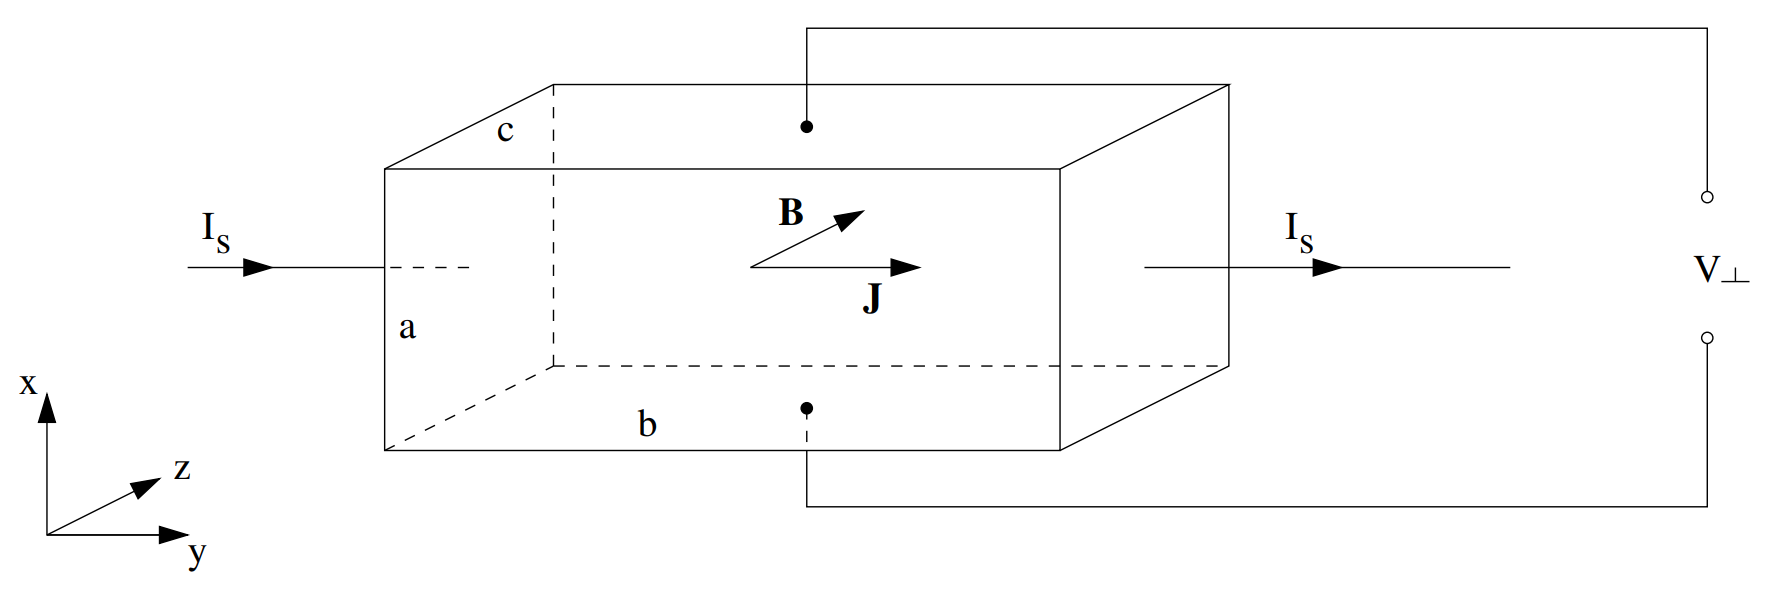
\includegraphics[width=.65\textwidth]{MaterialSetup.png}
            \label{fig:MaterialSetup}
        \end{center}
    \end{figure}
    By knowing all the other values, we can find values for $R_H$ and $\sigma$. \newline
    Since we are using germanium, which is a semiconductor, the definition for $R_H$ is slightly 
    different, it even depends on what type of charge carrier the semiconductor has. For p-type 
    semiconductors, which germanium is, the Hall coefficient is given by 
    \begin{equation}
        R_H=\frac{1.4}{n e}
        \label{eqn:Hall Coefficient p-type}
    \end{equation}
    with $e$ being the charge on an electron, $e=\SI{1.60217662e-19}{\coulomb}$. \newline
    \newline
    Now all this theory is based on the idea that the material in question stays at the same 
    temperature, since in semiconductors both the number of charges and their mobility within the 
    material are dependent on temperature. The problem is that as we drive a current through the 
    germanium, it is going to heat up thanks to Joule heating. \autoref{eqn:V Perp} and 
    \autoref{eqn:V parallel} are both linear, but since we expect values to change depending on 
    the temperature of the material, we can expect to see some deviation from linearity. 
    
    \section{Apparatus}\label{sec:Apparatus}
    \begin{itemize}
        \item DC power supply.
        \item 500 $\si{\ohm}$ resistor.
        \item Multimeter set to 200 mA scale.
        \item Multimeter set to 200 mV scale. 
        \item Multimeter set to 20 V scale. (All multimeters have $\pm 1\%$ error.)
        \item A piece of germanium. (See \autoref{fig:GermaniumDimensions}.)
        \item 
    \end{itemize}
    \begin{figure}[H]
        \begin{center}
            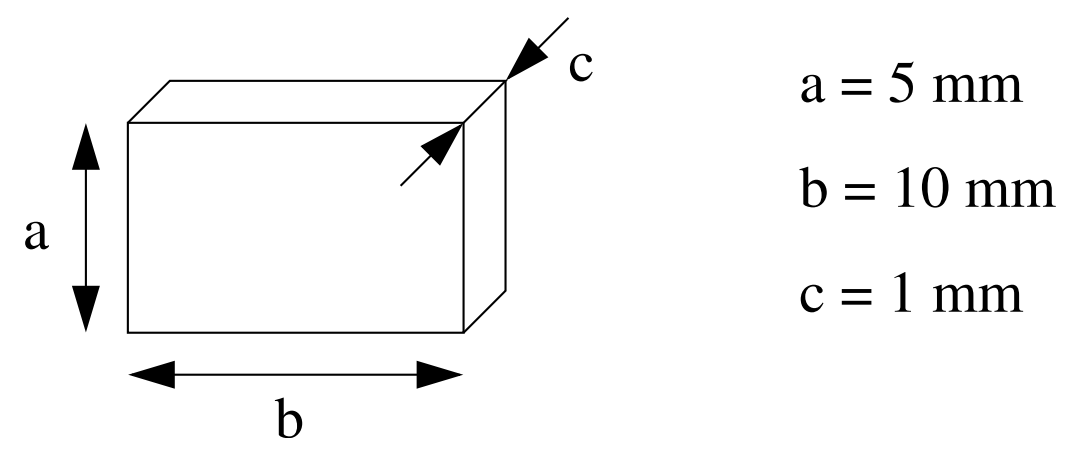
\includegraphics[width=.4\textwidth]{GermaniumDimensions.png}
            \caption{The dimensions of the sample of germanium used}
            \label{fig:GermaniumDimensions}
        \end{center}
    \end{figure}
    \begin{figure}[H]
        \begin{center}
            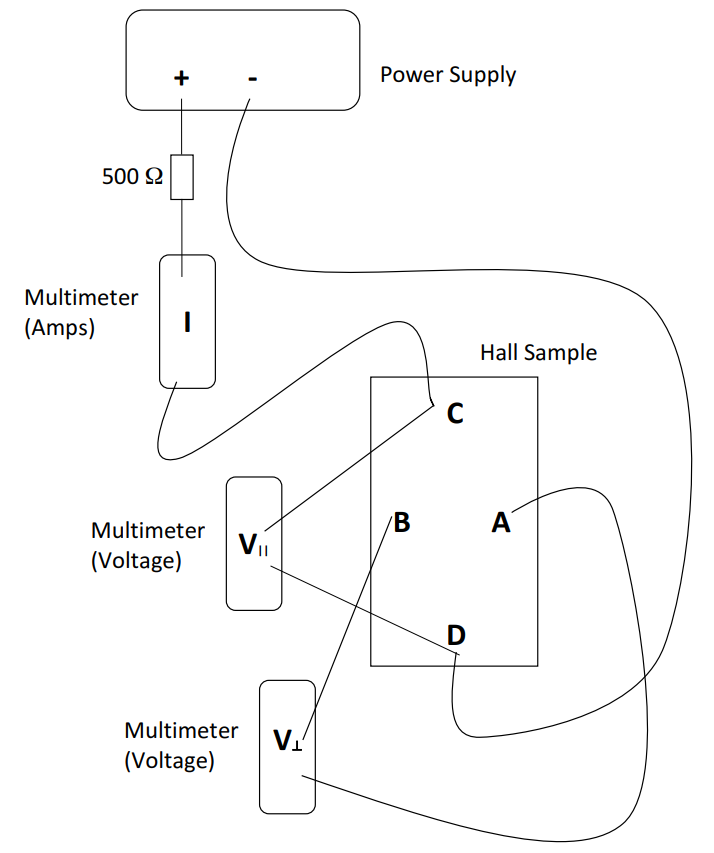
\includegraphics[width=.65\textwidth]{CircuitDiagram.png}
            \caption{The set-up of the circuit}
            \label{fig:CircuitDiagram}
        \end{center}
    \end{figure}
    
    

\end{document}